\documentclass[a4,11pt]{article}

\usepackage{./exercises}
\usepackage{./macros}
\usepackage{mathtools}
\usepackage{tikz}

\usepackage{graphicx}
\usepackage{ngerman}

\vltitel{Lineare Algebra 2}
\dozent{\small{Christian Haase}}
\assistent{\small{Jan Marten Sevenster}}
\tutoren{\small{%
    Theresa Graeber \\[-1ex] Eva Schinzel}}

\semester{Sommersemester 2023%
  % \raisebox{-10mm}[0pt][0pt]{%
  %   \parbox{0pt}{\includegraphics[width=27mm]{../../2015-ana1-L/Vorlesungsmaterial/ana1QR}}}
}

\DeclareMathOperator{\End}{End}
\DeclareMathOperator{\Span}{span}
% \DeclareMathOperator{\ker}{ker}
\DeclareMathOperator{\im}{im}
\newcommand{\bonusitem}{\item\hspace*{-2.4mm}*\ }


\begin{document}
\vspace*{-17mm}
{
\kopf
}
% \vspace*{-5mm}
% \enlargethispage*{25mm}

\newcounter{chapter}
\ueblatt{12}{ Montag, 17.~Juli 2023 um 10h00}


\begin{aufgabe}[4 Punkte]
Aus der Linearen Algebra 1 wissen wir, dass es f"ur jede lineare
Abbildung $F : V \to W$ des Rangs $r$ zwischen Vektorr"aumen der
Dimension $n$ respektive $m$ Basen $B_V$ und $B_W$ von $V$ und $W$
gibt, sodass die darstellende Matrix $M_{B_V}^{B_W}(F)$ von der Form
$$ \left( \begin{smallmatrix}
    E_r & 0_{r \times (n-r)} \\
    0_{(m-r) \times r} & 0_{(m-r) \times (n-r)}
  \end{smallmatrix} \right) \qquad \text{ ist.}$$
\begin{enumerate}
\addtocounter{enumi}{-1}
\bonusitem "Ubersetzen Sie diese Aussage (inklusive Quantoren(!)) in
die Sprache der Matrizen.
\item
Warum impliziert die Existenz dieser Basen nicht die Existenz der
Singul"arwertzerlegung von $M$?
\item
Kann mann umgekehrt aus der Singul"arwertzerlegung von $M$ direkt die
Existenz der oben beschriebene Basen folgern?
\end{enumerate}
\end{aufgabe}

\begin{aufgabe}[4 Punkte]
Wir betrachten das Internet (den gerichteten Graphen) %$(\{1, 2, 3,
                                %4\},\{(1, 2), (1, 3), (1, 4), (2, 3),
                                %(2, 4), (3, 1), (4, 1), (4, 3) \})$
\[
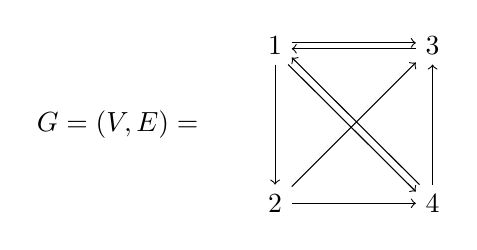
\begin{tikzpicture}
\node at (-2, 1) {$G = (V, E) = $};

\node (s3) at (2,2) {$3$};
\node (s4) at (2,0) {$4$};
\node (s2) at (0,0) {$2$};
\node (s1) at (0,2) {$1$};

\draw[->] (s1) -- (s2);
\draw[->] (s1.10) -- (s3.170);
\draw[->] (s1.305) -- (s4.145);

\draw[->] (s2) -- (s3);
\draw[->] (s2) -- (s4);

\draw[->] (s3.190) -- (s1.350);

\draw[->] (s4.125) -- (s1.325);
\draw[->] (s4) -- (s3);
\end{tikzpicture}
\]

Zu diesem Internet konstruieren wir die Link-Matrix $A$ wie in der
Vorlesung.
% Wir setzen
% \[
% A_{ji} = \begin{cases}
% 1 / \# \{ e \in E \mid e \text{ f"angt in } i \text{ an}\}, &
% \text{falls es ein } e \in E \text{  von } i \text{ nach } j \text{
% existiert} \\
% 0, & \text{ sonst.}
% \end{cases}
% \]

\begin{enumerate} \addtocounter{enumi}{-1}
\bonusitem Beschreiben Sie $E$ als Teilmenge von $V \times V$ und
bestimmen Sie $A$.
\item
Verifizieren Sie, dass Eig$(A;1)$ eindimensional ist.
\item
  \addtocounter{footnote}{1}
  Wir wollen den Pagerank manipulieren, ohne mit den Webmastern f"ur
  die Seiten $1$ bis $4$ zu reden. Dazu f"ugen wir ein Netz von fake
  Seiten ein, die sich untereinander verlinken und von denen einige
  auf die von uns pr"aferierte Seite $2$ verweisen.
  Wie "andert sich der Pagerank?\footnotemark
\item
  \addtocounter{footnote}{-1}
  Durch Zufall lernen wir Webmaster $4$ auf der Fachbereichsparty
  kennen. Wir k"onnen sie "uberzeugen, einen Link auf ihre Seite zu
  stellen, der auf eine unserer fake Seiten verweist. Wie "andert sich
  der Pagerank?\footnotemark
\end{enumerate}
\addtocounter{footnote}{-1}
\footnotetext{Im Tutorium oder in der Lerngruppe.}
\addtocounter{footnote}{1}
\footnotetext{Sie d"urfen ein Beispiel angeben, das die Situation
  illustriert, oder eine allgemeine Aussage ableiten und beweisen.}
\end{aufgabe}

\newpage

\begin{aufgabe}[4 Punkte]
Ein Spaziergang der L"ange $\ell \in \N$ in einem Internet $G=(V,E)$ ist
eine Folge von Seiten $v_0, \ldots, v_\ell \in V$ (Wiederholungen
erlaubt), so dass $(v_{i-1},v_i) \in E$ f"ur $i=1, \ldots, \ell$.

Zu einer Matrix $A \in M(n \times n; \R)$ mit ausschlie"slich nicht-negativen
Eintr"agen k"onnen wir ein Internet auf den Seiten $V = \{ 1, \ldots,
n \}$ definieren: $(i,j) \in E :\Leftrightarrow a_{ij} > 0$.

Zeigen Sie, dass f"ur $i,j \in V$ der $ij$-Eintrag der $\ell$-ten
Potenz $A^\ell$ genau dann positiv ist, wenn es in $G=(V,E)$ einen
Spaziergang der L"ange $\ell$ von $j$ nach $i$ gibt.
  
\end{aufgabe}

\end{document}

%%% Local Variables: 
%%% mode: latex
%%% End: 
